%%%%%%%%%%%%%%%%%%%%%%%%%%%%%%%%%%%%%%%%%%%%%%%%%%%%%%%%%%%%%%%%%%
% The following comments were written in Portuguese, because this 
% template applies only for School of Technology at University 
% of Campinas, Brazil.
%
% Este é um modelo Latex para monografias de Trabalhos de Conclusão 
% de Curso (TCC) na graduação, monografias de Mestrado e Teses de 
% doutorado da Faculdade de Tecnologia (FT) da Universidade 
% Estadual de Campinas (UNICAMP).
%
% Esse modelo e seu respectivo arquivo de classe de documento 
% foram adaptado do modelo de teses e dissertações do 
% Instituto de Computação da UNICAMP.
%
% Autor: André Leon Sampaio Gradvohl, Dr.
% Email:        gradvohl@ft.unicamp.br
% Lattes CV:    http://lattes.cnpq.br/9343261628675642
% ORCID:        0000-0002-6520-9740
% 
% Última versão: 24/Março/2019
%
% Adições/Alterações nesta última versão 
% - Alteração da fonte padrão (times) para fonte libertine, mais 
%   adequada do que a Times New Roman para teses, mas ainda
%   compatível com a times.
% - Adição de comandos para abreviações especiais, e.g., i.e. e
%   p.ex., respectivamente \eg , \ie , \pex
% - Adição do pacote booktabs para tabelas.
% - Ajustes nas referências bibliográficas de acordo com a norma 
%   ABNT NBR 6023 de 14/11/2018.
%%%%%%%%%%%%%%%%%%%%%%%%%%%%%%%%%%%%%%%%%%%%%%%%%%%%%%%%%%%%%%%%%%
%
% Escolha: Portugues ou Ingles ou Espanhol.
% Para a versão final do texto, acrescente a palavra "Final",
% como na segunda linha abaixo da próxima.
%\documentclass[Portugues]{tese-FT}
\documentclass[Portugues,Final]{tese-FT}
%\documentclass[Ingles]{tese-FT}
%\documentclass[Espanhol,Final]{tese-FT}

%Adicione seu arquivo com as referências bibliográficas
\addbibresource{bibliografia.bib}

%O pacote a seguir gera um dummy text. Elimine a linha quando
% for editar seu texto.
%\usepackage{lipsum}

\usepackage{soul}
\usepackage{cancel}
\newcommand\tab[1][1cm]{\hspace*{#1}}
\usepackage{amsmath}
\usepackage{minted}
\usepackage{booktabs}

% Adicione o pacote a seguir, se seu texto tiver uma lista de 
% símbolos. Não confunda com a lista de abreviaturas.
%\usepackage[symbols,nogroupskip,sort=none]{glossaries-extra}

\begin{document}

% Escolha entre autor ou autora:
\autor{Pedro Henrique Neves dos Santos}
%\autora{Nome da Autora}

% Sempre deve haver um título em português:
\titulo{IT306W - Fluxo de carga completo}

% Se a língua for o inglês ou o espanhol defina:
%\title{The Dissertation or Thesis Title in English or Spanish for FT}

% Escolha entre orientador ou orientadora e inclua os títulos:
\orientador{Prof. Dr. Nome do Orientador}
%\orientadora{Profa. Dra. Nome da Orientadora}

% Escolha entre coorientador ou coorientadora, se houver, 
% e inclua os títulos:
%\coorientador{Prof. Dr. Eng. Lic. Nome do Co-Orientador}
%\coorientadora{Prof. Dra. Eng. Lic. Nome da Co-Orientadora}

% Escolha entre uma das quatro opções a seguir (comente as demais):
%\bsi         % para Trabalho de Conclusão de Curso em BSI
%\tads       % para Trabalho de Conclusão de Curso em TADS
%\qualificacaoMestrado  % Para textos de qualificação de mestrado.
%\qualificacaoDoutorado % Para textos de qualificação de doutorado.
\mestrado   % para Dissertação de Mestrado em Tecnologia
%\doutorado  % para Tese de Doutorado em Tecnologia

%Defina a área de concentração. Se for TCC, deixe comentado
\areaConcentracao{Sistemas de Informação e Comunicação}
%\areaConcentracao{Ambiente}
%\areaConcentracao{Ciência dos Materiais}

% Se houve cotutela, defina:
%\cotutela{Universidade Nova de Plutão}

%Defina a data da defesa no formato {Dia}{Mês}{Ano}
\datadadefesa{13}{05}{2020}

% Para a versão final defina:
% Repita o nome do Orientador(a) no primeiro avaliador
%\avaliadorA{Prof. Dr. Nome do Orientador}{FT/UNICAMP}
%\avaliadorB{Profa. Dra. Segunda Avaliadora}{Instituição da segunda avaliadora}
\avaliadorC{Dr. Terceiro Avaliador}{Instituição do terceiro avaliador}
% \avaliadorD{Prof. Dr. Quarto Avaliador}{Instituição do quarto avaliador}
% \avaliadorE{Prof. Dr. Quinto Avaliador}{Instituição do quinto avaliador}
% \avaliadorF{Prof. Dr. Sexto Avaliador}{Instituição do sexto avaliador}
% \avaliadorG{Prof. Dr. Sétimo Avaliador}{Instituição do sétimo avaliador}
% \avaliadorH{Prof. Dr. Oitavo Avaliador}{Instituição do oitavo avaliador}


% Para incluir a ficha catalográfica em PDF na versão final, 
% copie o arquivo PDF, descomente e ajuste a linha a seguir:
%\fichacatalografica{arquivo.pdf}

% Este comando deve ficar aqui:
\paginasiniciais
% Sempre deve haver um resumo em português:
\begin{resumo}

%Primeiro trabalho apresentado \`a disciplina IT306.\\\\\
H\'a muitas d\'ecadas, a energia el\'etrica desempenha um papel vital na nossa sociedade. Desde necessidades mais simples, como ilumina\c{c}\~ao p\'ublica, at\'e necessidades mais complexas, como equipamentos m\'edicos e industrias inteiras, s\'o s\~ao fact\'iveis pois temos energia el\'etrica. E ela \'e est\'avel.\\
Para que isso seja poss\'ivel, \'e necess\'ario alguma metodologia que nos forne\c{c}a o estado atual do sistema para que se possa, ent\~ao, atuar apropriadamente.\\
Neste trabalho faremos um estudo sobre sobre fluxo de potência, uma metodologia que nos fornece tens\~oes nodais e angulos de fase.



\end{resumo}


% A lista de símbolos é opcional. Não confunda a lisa de símbolos
% com a lista de abreviaturas.
\prefacesection{Lista de Símbolos}

% Coloque o símbolo na primeira coluna e a 
% descrição na segunda coluna. Use descrições
% rápidas.

\begin{table}[!ht]
  \begin{tabular}{p{3cm}l}
	$NB$        & N\'umero de Barras \\
	$k$       & Inteiro entre 1 e $NB$\\
	$m$        & N\'umero de Barras \\
	$\in$       & Inteiro entre 1 e $NB$\\
	$\kappa$        & Conjunto formado pela barra $k$ e todas as barras $m$ conectadas ela \\
	$G_{km}$       & Inteiro entre 1 e $NB$\\
	$B_{km}$        & N\'umero de Barras \\
	$k$       & Inteiro entre 1 e $NB$\\
	
	$c$       & Descrição do símbolo $c$ 
  \end{tabular}
\end{table}

% A lista de abreviações e siglas vem a seguir.
% Dê uma olhada no pacote nomencl para ver os comandos para 
% adicionar abreviações e siglas no texto.
\renewcommand{\nomname}{Lista de Abreviações e Siglas}
\printnomenclature[3cm]


% O sumário vem aqui:
\tableofcontents
\fimdaspaginasiniciais


% O corpo da dissertação ou tese começa aqui:
%
% O comando a seguir inclui o arquivo introducao.tex
% que contém o capítulo de Introdução. 
% Detalhe: não precisa incluir a extensão .tex
%\include{introducao}


\chapter{Introdu\c{c}\~ao e teoria}

%\section{Motiva\c{c}\~ao}

% DIZER ALGO SOBRE COMO SERA O SISTEMA, COM BARRAS E CONEXOES E QUE FICA COMPLEXO SEM ANALISE DE FLUXO DE CARGA Mas como \'e possivel garantir o planejamento e opera\c{c}\~ao sistema de grandes propor\c{c}\~oes como esse? Para isso, \'e preciso saber o estado atual do sistema. Por\'em, n\~ao \'e vi\'avel medir todos os pontos de interesse. Isso seria custoso e tomaria muito tempo. 


%Para  como um todo \'e necessario que tenhamos ferramentas que nos ajudem a estimar o estado da rede 

%\section{Introdução à Teoria}
A ferramenta de an\'alise de sistemas de energia el\'etrica aqui discutida ser\'a a An\'alise de Fluxo de Pot\^encia. Essa an\'alise nos fornecer\'a um metodo de cálculo de importantes grandezas de todo o sistema, a partir de algumas grandezas conhecidas, ou seja, que podem ser medidas. Esta \'e uma ferramenta aplicada \`a um sistema est\'atico. \cite{monticelli}
\section{Modelagem}
\label{SectionIntro}
Toda a rede ser\'a composta por ramos e barras, onde ramos s\~ao a representa\c{c}\~oes das linhas de transmiss\~ao e transformadores. As barras s\~ao n\'os do sistema e nesses pontos de interesse, pode-se medir fisicamente algumas grandezas, a depender do tipo de barra. S\~ao definidas quatro vari\'aveis \`a para cada k-ésima barra, correspondentes \`a tens\~ao e \`a inje\c{c}\~ao de
pot\^encia nesta barra, $V_k$, magnitude da tens\~ao nodal, $\theta_k$ angulo da tens\~ao nodal, $P_k$ inje\c{c}\~ao l\'iquida de pot\^encia ativa e $Q_k$ inje\c{c}\~ao l\'iquida de pot\^encia reativa. As barras s\~ao divididas em categorias como na tabela \ref{t_PQPVSlack} de acordo com as grandezas conhecidas e suas incognitas.
\begin{table}[]
\caption{Categoria das barras de acordo com variáveis conhecidas}
\begin{tabular}{@{}llll@{}}
\toprule
Tipo & Dados & Incógnitas & Caracteristicas \\ 
\midrule
$PQ$ & $P_k$,$Q_k$ & $V_k$,$\theta_k$  & Barra de carga \\
$PV$ & $P_k$,$V_k$ & $Q_k$,$\theta_k$  & Barra de geração\\
Referência (Slack) & $V_k$,$\theta_k$ & $P_k$,$Q_k$& Barra de geração em grandes fornecedoras \\ \bottomrule
\end{tabular}
\label{t_PQPVSlack}
\end{table}



\section{Formula\c{c}\~ao do problema b\'asico}
\label{SectionFormula}
\subsection{Injeção de potências}

Seja uma rede de energia gen\'erica que cont\'em um n\'umero de barras \textit{(NB)} arbitr\'ario. Para cada barra, \'e poss\'ivel escrever duas equa\c{c}\~oes de inje\c{c}\~oes de pot\^encia, como em \ref{Pk} e \ref{Qk}. Elas são obtidas ao aplicar Lei de Kirchhoff das correntes em todas as $NB$ barras do sistema.\\
\begin{equation}
    P_k = V_k \sum_{m\in \kappa} V_m (G_{km} cos\theta_{km} + B_{km}sen\theta_{km})
    \label{Pk}
\end{equation}
\begin{equation}
    Q_k = V_k \sum_{m\in \kappa} V_m (G_{km} sen\theta_{km} - B_{km}cos\theta_{km})
    \label{Qk}
\end{equation}
Portanto, em um sistema com \textit{NB} barras, \'e possivel obter $2.NB$ equa\c{c}\~oes.\\
Neste problema, utilizaremos como variáveis de estado, ou seja, nosso conjunto de incognitas que descreverão o sistema, as variáveis $V$ e $\theta$, representados em \ref{Vs} e \ref{TetaS}. Com esses valores resolvidos, \'e possível calcular todas as injeções de potência em todas as barras.\\
\begin{equation}
    V^S  = \left[ \begin{matrix} V_1^S & V_2^S & V_3^S & ... & V_{NB}^S  \end{matrix} \right]^T 
    \label{Vs}
\end{equation}

\begin{equation}
    \theta^S  = \left[ \begin{matrix} \theta_1^S & \theta_2^S & \theta_3^S &... & \theta_1^S  \end{matrix} \right]^T 
    \label{TetaS}
\end{equation}
Quando \ref{Vs} e \ref{TetaS} forem resolvidas, será possivel aplicar em \ref{Pk} e \ref{Qk} para se obter \ref{Pk_s} e \ref{Qk_s}, que será as injeções de potência para o estado atual da rede.
\begin{equation}
    P_k = V_k^S \sum_{m\in \kappa} V_m^S (G_{km} cos\theta_{km}^S + B_{km}sen\theta_{km}^S)
    \label{Pk_s}
\end{equation}
\begin{equation}
    Q_k = V_k^S \sum_{m\in \kappa} V_m^S (G_{km} sen\theta_{km}^S - B_{km}cos\theta_{km}^S)
    \label{Qk_s}
\end{equation}
Problema consiste em obter o estado $(V^S,\theta^S)$.\\
Com um simples algebrismo matemático, as equações \ref{Pk} e \ref{Qk} serão representas aqui como em \ref{Pk_balanceado} e \ref{Qk_balanceado}.
\begin{equation}
    P_k - V_k \sum_{m\in \kappa} V_m (G_{km} cos\theta_{km} + B_{km}sen\theta_{km}) = 0
    \label{Pk_balanceado}
\end{equation}
\begin{equation}
    Q_k - V_k \sum_{m\in \kappa} V_m (G_{km} sen\theta_{km} - B_{km}cos\theta_{km}) = 0
    \label{Qk_balanceado}
\end{equation}

%essas equaoces tem que dar 0 pois são dua coisas iguais

%dada uma rede qualquer, o nume de equacoes sera XXXX colocar 

%inserir tahbelas tipos de barras

%numero de equacoes = numero de incognitas e o sistema é LI. POrtante há solução

%do ponto de vista didático

\subsection{Matriz de Admitância}
Seja a matriz de admitância nodal $Y$ e ela se relacione com o vetor de tensões nodais $V$ e vetor de injeções de corrente nodais $I$ da forma como em \ref{Admitancia}.
\begin{equation}
    I = Y.V
    \label{Admitancia}
\end{equation}
A regra de formação dessa matriz $Y$ será dada por \ref{AdmitanciaElementosForaDiagonal} e \ref{AdmitanciaElementosDiagonal} (A dedução desse conjunto de formulas não será abordado neste trabalho).\\
A dimensão da matriz $Y$ será de $NB$x$NB$.\\
Para os elementos fora da diagonal principal, será o valor negativo da admitância série entre as duas barras, como em \ref{AdmitanciaElementosForaDiagonal}.
\begin{equation}
    Y_{km} = -y_{km}
    \label{AdmitanciaElementosForaDiagonal}
\end{equation}
Para os elementos na diagonal principal, será a soma das admitâncias conectadas à barra, como em \ref{AdmitanciaElementosDiagonal}, onde $\Omega_k$ é o conjunto de barras vizinhas da barra $k$.
\begin{equation}
    Y_{kk} = \sum_{m\in \Omega_k} \left(y_{km} + j\frac{b^{sh}_{km}}{2}\right)
    \label{AdmitanciaElementosDiagonal}
\end{equation}
Ainda, a matriz $Y$ será dividida em parte real(\ref{G}) e parte imaginária (\ref{B}). Dando origem às matrizes de condutância $G$ e susceptância $B$, usadas nas equações de injeção de potência \ref{Pk} e \ref{Qk}.
\begin{equation}
    G = \mathbb{R} (Y)
    \label{G}
\end{equation}
\begin{equation}
    B = \mathbb{I} (Y)
    \label{B}
\end{equation}



%\subsection{Subsistema 1}
%calcular v e teta faltando

%na barra de ref não falta nenhum
%na barra PQ falta 2 variaveis V e teta
%na barrade geraç~]a., PV, já conheco V, só falta teta


%grandezas conhecidas 
%2NPQ + NPV grandezas

%problemas tem solução

%como serao as equacçoes. Serão eq de injeções de pot ativa e reativa

%P espeficada 
%valor especificado na barra k - valor calculado = 0 

%\subsection{Subsistema 2}
%calcula P e Q faltando

%conhecendo os V e Tetas, calcula-se P e Q
%na barra PV vc calcula só Q
%na barra slack vc calcula P e Q

\section{Formula\c{c}\~ao do m\'etodo de Newton}
\label{SectionNewton}
O algoritmo de Newton é um método para calcular os zeros de funções reais de uma variável reais. Baseando em uma aproximação inicial arbitraria, $x^{(1)}$, tem-se \ref{Newton} para $n>1$. \cite{newton}
\begin{equation}
    x^{x+1} = x^{n} - \frac{f(x^{(n)}}{f'(x^{(N)}} = x^{n} - \Delta x
    \label{Newton}
\end{equation}
Fazendo $\Delta x = \frac{f(x^{(n)}}{f'(x^{(N)}}$ 
\begin{equation}
    x^{x+1} = x^{n} - \Delta x
    \label{Newton_Delta}
\end{equation}
\subsection{Aplicação do método de Newton em problemas de Fluxo de Potência}
Para solucionar o problema do Fluxo de Potência utilizando o método de Newton, é necessário estabelecer equações que relacionem o problema na forma de $f(x)=0$. A forma mais adequada, é utilizando as equações que modelam o balanceamento das injeções de potência \ref{Pk_balanceado} e \ref{Qk_balanceado}, mas desta vez elas não vão a $0$, pois ainda não estão resolvidas. Neste momento, igualaremos elas um $\Delta$, que é tão próximo de $0$ quanto se queira, como descrito nas equações \ref{Pk_balanceado_delta} e \ref{Qk_balanceado_delta}.\\
\begin{equation}
    \Delta P_k = P^{esp}_k - P^{calc}_k(V,\theta)= P^{esp}_k - V_k \sum_{m\in \kappa} V_m (G_{km} cos\theta_{km} + B_{km}sen\theta_{km})
    \label{Pk_balanceado_delta}
\end{equation}
\begin{equation}
    \Delta Q_k = Q^{esp}_k - Q^{calc}_k(V,\theta) = Q^{esp}_k - V_k \sum_{m\in \kappa} V_m (G_{km} sen\theta_{km} - B_{km}cos\theta_{km})
    \label{Qk_balanceado_delta}
\end{equation}
Onde:
\begin{itemize}
    
    \item $P^{esp}_k = P^G_k -P^C_k$ e $Q^{esp}_k = Q^G_k -Q^C_k$ que são os valores das injeções de potência ativa e reativa especificados para as barras.
    \item $P^{calc}_k(V,\theta)$ e $Q^{calc}_k(V,\theta)$ são calculados através das equações das potências nodais.
    \item $\Delta P_k$ e $\Delta Q_k$ são chamados de mismatches ou resíduos de potência ativa e reativa. 

\end{itemize}
Em termos práticos, para a resolução do sistema de equações $g(x) = 0$ pelo método de Newton, é necessário a determinação do vetor de correção do estado $\Delta x$ a cada iteração. Para cada iteração  $\nu$, $\Delta x$ é obtido através de \ref{Newton_aplicado} e verificado se a convergência ocorreu, isto é, se $|\Delta_x| < Tol$.\\
\begin{equation}
    g(x^\nu) = -J(x^\nu) . \Delta (x^\nu)
    \label{Newton_aplicado}
\end{equation}
Onde:\\
\begin{equation}
   g(x^\nu) = \left[ \begin{matrix} \Delta P^\nu \\ \Delta Q^\nu  \end{matrix} \right] 
    \label{g_x_nu}
\end{equation}
\begin{equation}
   \Delta (x^\nu) = \left[ \begin{matrix} \Delta \theta^\nu \\ \Delta V^\nu  \end{matrix} \right] 
    \label{delta_x_nu}
\end{equation}
\begin{equation}
   J (x^\nu) = - \left[ \begin{matrix} \frac{\partial (P)}{\partial \theta} & \frac{\partial (P)}{\partial V}  \\ \frac{\partial (Q)}{\partial \theta} & \frac{\partial (Q)}{\partial V}  \end{matrix} \right] 
    \label{Jacobiana}
\end{equation}
As submatrizes que compõem a matriz Jacobiana \ref{Jacobiana} são geralmente representadas por \ref{H}, \ref{N}, \ref{M} e \ref{L} e são obtidas equações das potências nodais \ref{Pk} e \ref{Qk}
\begin{equation}
   H = \frac{\partial (P)}{\partial \theta}
    \label{H}
\end{equation}
\begin{equation}
   N = \frac{\partial (P)}{\partial V}
    \label{N}
\end{equation}
\begin{equation}
   M = \frac{\partial (Q)}{\partial \theta}
    \label{M}
\end{equation}
\begin{equation}
   L = \frac{\partial (Q)}{\partial V}
    \label{L}
\end{equation}
Resultando em \ref{HNML_eq}.
\begin{equation}
    \left[ \begin{matrix} \Delta P^\nu \\ \Delta Q^\nu  \end{matrix} \right]  = \left[ \begin{matrix} H & N \\ M & L  \end{matrix} \right]^\nu . \left[ \begin{matrix} \Delta \theta^\nu \\ \Delta V^\nu  \end{matrix} \right] 
    \label{HNML_eq}
\end{equation}
As mastrizes H, N, M e L podem ter seus valores calculados utilizando as equações \ref{H_resolvido}, \ref{N_resolvido}, \ref{M_resolvido} e \ref{L_resolvido}.(As deduções das matrizes H, N, M e L podem ser encontradas em livros didáticos e, portanto, serão omitidas neste trabalho).\\

\begin{equation}
  \left\{    \begin{array}{lll}
                H_{kk} = \frac{\partial (P_k)}{\partial \theta_k} = -B_{kk}V_k^2 - V_k\sum_{m\in \kappa} V_m(G_{km} sen\theta_{km} - B_{km}cos\theta_{km})\\
                H_{km} = \frac{\partial (P_k)}{\partial \theta_m} = V_k V_m (G_{km} sen\theta_{km} - B_{km}cos\theta_{km})\\
                H_{mk} = \frac{\partial (P_k)}{\partial \theta_k} =-V_k V_m (G_{km} sen\theta_{km} + B_{km}cos\theta_{km})
            \end{array}\right.
    \label{H_resolvido}
\end{equation}

\begin{equation}
  \left\{    \begin{array}{lll}
                N_{kk} = \frac{\partial (P_k)}{\partial V_k} = G_{kk}V_k \sum_{m\in \kappa} V_m(G_{km} cos\theta_{km} + B_{km}sen\theta_{km})\\
                N_{km} = \frac{\partial (P_k)}{\partial V_m} = V_k(G_{km} cos\theta_{km} + B_{km}sen\theta_{km})\\
                N_{mk} = \frac{\partial (P_m)}{\partial V_k} =V_m(G_{km} cos\theta_{km} + B_{km}sen\theta_{km})
            \end{array}\right.
    \label{N_resolvido}
\end{equation}

\begin{equation}
  \left\{    \begin{array}{lll}
                M_{kk} = \frac{\partial (Q_k)}{\partial \theta_k} = -G_{kk}V_k^2 + V_k\sum_{m\in \kappa} V_m(G_{km} cos\theta_{km} + B_{km}sen\theta_{km})\\
                M_{km} = \frac{\partial (Q_k)}{\partial \theta_m} = -V_k V_m (G_{km} cos\theta_{km} + B_{km}sen\theta_{km})\\
                M_{mk} = \frac{\partial (Q_m)}{\partial \theta_k} =-V_k V_m (G_{km} cos\theta_{km} - B_{km}sen\theta_{km})
            \end{array}\right.
    \label{M_resolvido}
\end{equation}

\begin{equation}
  \left\{    \begin{array}{lll}
                L_{kk} = \frac{\partial (Q_k)}{\partial V_k} = -B_{kk}V_k +\sum_{m\in \kappa} V_m(G_{km} sen\theta_{km} - B_{km}cos\theta_{km})\\
                L_{km} = \frac{\partial (Q_k)}{\partial V_m} = V_k(G_{km} sen\theta_{km} - B_{km}cos\theta_{km})\\
                L_{mk} = \frac{\partial (Q_m)}{\partial V_k} =-V_m (G_{km} sen\theta_{km} + B_{km}cos\theta_{km})
            \end{array}\right.
    \label{L_resolvido}
\end{equation}

\section{Algoritmo implementado}

Aqui será utilizado um algoritmo discutido nos slides do Professor Castro. \cite{castro}.

\begin{enumerate}
    \item   O contador de iterações é inicializado $\nu = 0$.   Escolhe-se condições de contorno iniciais para as magnitudes das tensões nodais nas barras $PQ$ e ângulos de fase das tensões nodais nas barras $PQ$ e $PV$, onde não houver esse valor previamente estabelecido.
            O vetor $x$ pode ser montado como em \ref{X}.
            \begin{equation}
            x  = \left[ \begin{matrix} \theta^0 & V^0  \end{matrix} \right]^T 
            \label{X}
            \end{equation}
    \item   Calcula-se $P_k(V_\nu, \theta)$ para as barras $PQ$ e $PV$.\\
            Calcula-se $Q_k(V_\nu, \theta_\nu)$ para as barras $PQ$.
            Calcula-se os respectivos mismatches de potência \ref{delta_x_nu}.
    \item   Testa-se a convergência: Se $max \{|\Delta P_k^\nu|\}_k=PQ$ , $PV\leq \varepsilon P$ e $max \{|\Delta Q_k^\nu|\}_k=PQ \leq \varepsilon P$\\
            Então processo iterativo convergiu para a solução $[\theta ^\nu V^\nu]^T$. Pular para o passo $7$.\\
            Senão, prosseguir para passo $4$.
    \item   Calcula-se a matriz Jacobiana como em \ref{Jacobiana}
    \item   Calcula-se as correções resolvendo o sistema \ref{HNML_eq} e determina-se nova solução $(V^{\nu + 1},\theta^{\nu + 1})$
    \item   Incrementa-se contador de iterações $\nu = \nu + 1$ e volta-se ao passo 2.
    \item   Calcula-se $P_k$ para a barra de referência e $Q_k$ para as barras de referência e $PV$.
\end{enumerate}



\chapter{Estudos de caso}
\label{SectionEstudosDeCaso}
Neste capítulo, será estudado uma rede elementar (na seção \ref{SectionRedePequena}) e XXXXXXXXXXXXX redes maiores. Neste trabalho, a rede elementar tem um papel fundamental para compreensão de cada iteração do método, além de servir como calibração e teste para todas as modificações subsequentes. Para cada modificação no código de referência, ainda que pequena, deve ser retestado tendo a saída desta rede como parâmetro.
\section{Rede de 2 barras e 1 linha de transmissão}
\label{SectionRedePequena}
Considere a rede de duas barras e uma linha de transmissão \ref{FigRede2barras1linha}. Esse é o exemplo mais simples possível e foi apresentado e resolvido nos slides de aula.\\
\begin{figure}[!htb]
\caption{Rede de duas barras e uma linha de transmissão}
 \centering % para centralizarmos a figura
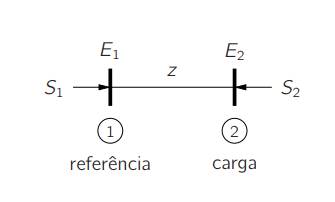
\includegraphics[width=8cm]{figuras/rede2barras1linha.PNG} 
\label{FigRede2barras1linha}
\end{figure}

\begin{equation}
Dados \left\{    \begin{array}{lll}
                E_1=1,0112	\angle 0^o pu\\
                z = 0,01+j0,05 pu\\
                S_2 = -(1,0+j0) pu
            \end{array}\right.
    \label{rede1_dados}
\end{equation}
\subsection{Equacionamento}
A matriz admitância será dada por \ref{rede1_Admitância}, que foi calculado com as regras \ref{AdmitanciaElementosForaDiagonal} e \ref{AdmitanciaElementosDiagonal}.
\begin{equation}
   Y = \left[ 
    \begin{matrix} 
        3,8462-j19,2308 & -3,8462+j19,2308  \\ 
        -3,8462+j19,2308 & 3,8462-j19,2308  
    \end{matrix} \right] 
    \label{rede1_Admitância}
\end{equation}
Portanto, tem-se as equações nodais $P_2$ e $Q_2$ em \ref{PeQ_resolvidos}. As incognitas são $\theta_2$ e $V_2$
\begin{equation}
    \left\{    \begin{array}{lll}
                P_2= V_2V_1(G_{21}cos \theta_{21}+ B_{21}sen \theta_{21}) + V^2_2G_{22}\\
                Q_2= V_2V_1(G_{21}sen \theta_{21}- B_{21}cos \theta_{21}) - V^2_2B_{22}
            \end{array}\right.
    \label{PeQ_resolvidos}
\end{equation}
Portanto, as equações de fluxo serão \ref{PeQ_esp}
\begin{equation}
    \left\{    \begin{array}{lll}
                P^{esp}_2-P_2 = -1-P_2=0\\
                Q^{esp}_2-Q_2 = 0-Q_2=0
            \end{array}\right.
    \label{PeQ_esp}
\end{equation}
Por fim, monta-se as equações linearizadas de fluxo de carga em \ref{FluxoLinearizado}.
\begin{equation}
   \left[ \begin{matrix} \Delta P_2 \\ \Delta Q_2  \end{matrix} \right] =  \left[ \begin{matrix} \frac{\partial (P_2)}{\partial \theta_2} & \frac{\partial (P_2)}{\partial V_2}  \\ \frac{\partial (Q_2)}{\partial \theta_2} & \frac{\partial (Q_2)}{\partial V_2} \end{matrix} \right] .  \left[ \begin{matrix} \Delta \theta_2 \\ \Delta V_2  \end{matrix} \right]
    \label{FluxoLinearizado}
\end{equation}
Onde, a partir de \ref{H_resolvido}, \ref{N_resolvido}, \ref{M_resolvido} e \ref{L_resolvido}, tem-se \ref{HMNL_resolvidoRedePequena}.
\begin{equation}
  \left\{    \begin{array}{llll}
                \frac{\partial (P_2)}{\partial \theta_2} =-V_2 V_1 (G_{21} sen\theta_{21} - B_{21}cos\theta_{21})\\
                \frac{\partial (P_2)}{\partial V_2} =V_1(G_{21} cos\theta_{21} + B_{21}sen\theta_{21}) + 2V_2G_{22}\\
                \frac{\partial (Q_2)}{\partial \theta_2} = V_2 V_1 (G_{21} cos\theta_{21} + B_{21}sen\theta_{21})\\
                \frac{\partial (Q_2)}{\partial V_2} =-V_1 (G_{21} sen\theta_{21} - B_{21}cos\theta_{21})
            \end{array}\right.
    \label{HMNL_resolvidoRedePequena}
\end{equation}
\subsubsection{Processo iterativo $\nu=0$}
Para a primeira iteração ($\nu=0$), tem-se:
\begin{equation}
  \left\{    \begin{array}{llll}
                V_2=1pu\\
                \theta_2=0
    \end{array}\right.
\label{RedePequenaItera0a}
\end{equation}
\begin{equation}
    \left\{    \begin{array}{llll}
                P_2= -0,0431\\
                \Delta P_2 = -0,9569\\
                Q_2 = -0,2154\\
                \Delta Q_2 = 0,2154
            \end{array}\right.
    \label{RedePequenaItera0b}
\end{equation}
Como os mismatches ainda são maiores que a tolerância, atualiza-se o estado, incrementa-se $\nu=\nu+1$. A nova matriz Jacobiana ficará com \ref{JRedePequena}.
\begin{equation}
   J = \left[ 
    \begin{matrix} 
        19,4462 & 3,8031  \\ 
        -3,8031 & 19,0154  
    \end{matrix} \right] 
    \label{JRedePequena}
\end{equation}
\subsubsection{Processo iterativo $\nu=1$}
Para a segunda iteração ($\nu=1$), tem-se:
\begin{equation}
  \left\{    \begin{array}{llll}
                P_2= -0,9960\\
                \Delta P_2 = -0,0040\\
                Q_2 = 0,0240\\
                \Delta Q_2 = -0,0240
            \end{array}\right.
    \label{RedePequenaItera1}
\end{equation}
Como os mismatches ainda são maiores que a tolerância, atualiza-se o estado, incrementa-se $\nu=\nu+1=2$. A nova matriz Jacobiana ficará com \ref{JRedePequena2}.
\begin{equation}
   J = \left[ 
    \begin{matrix} 
        19,2535 & 2,8560  \\ 
        -4,8515 & 19,2781
    \end{matrix} \right] 
    \label{JRedePequena2}
\end{equation}
\subsubsection{Processo iterativo $\nu=2$}
Para a terceira iteração ($\nu=2$), tem-se:
\begin{equation}
  \left\{    \begin{array}{llll}
                P_2= -1\\
                \Delta P_2 = 0\\
                Q_2 = 0\\
                \Delta Q_2 = 0
            \end{array}\right.
    \label{RedePequenaItera2}
\end{equation}
Como os mismatches são menores que a tolerância, o método convergiu.
\subsubsection{Calculo de $E_2$}
Pela equação de potência na barra $2$, tem-se \ref{RedePequenaPotBarra2}.
\begin{equation}
    S_1 = E_1.I^*_12=E1.[\frac{1}{Z}.(E_1-E_2]^*= 1.01+j0,05pu
    \label{RedePequenaPotBarra2}
\end{equation}
Resumo das iterações está aprensentado na tabela \ref{t_redePequenaResumo}.
\begin{table}[!htb]
\centering
\caption{Resumo das iterações da rede}
\begin{tabular}{lll}
\hline
Iteração & $E_2$          & $E_2$ \\ \hline
0        & 1+j0           & $1\angle 0^o$ \\
1        & 1-j0,0494      & $1 \angle -2.84^o$ \\
2        & 0,09988-0,0495 & $1 \angle -2,8^o$ \\ \hline
\end{tabular}
\label{t_redePequenaResumo}
\end{table}

\subsection{Solução por software}
Com os dados \ref{rede1_dados} é possivel montar os \textit{arrays} no código abaixo. Eles serão usados como \textit{inputs} do código utilizado neste trabalho. 
\begin{minted}[mathescape, style = autumn,
    frame = single, fontsize=\footnotesize]{matlab}
nome_da_rede = 'Rede de 2 barras e 1 ramos - Demostração do Slide';
baseMVA      = 1 ; % MVA - Os dados do problema já estavam em pu
%Núm-Tipo-V-Âng-Pg-Qg-Pc-Qc-bshk % (PU/Graus) - 3ref; 2PV; 0PQ
barras = [1 3 1.0112 0 0 0 00.0 0 0
          2 0 0.0000 0 0 0 -1.0 0 0 ];
ramos  = [1 2 0.01 0.05 0.0 1.0 0.0 ];%De-Para-r-x-bshl-tap-fi
\end{minted}
A saída dessa rede, calculado pelo algoritmo descrito no capítulo \ref{SectionCodigo}, é dado nos blocos de código a seguir.
Nesse bloco temos a formação da matriz de admitância. É a mesma matriz calculada em \ref{rede1_Admitância}, como esperado.
\begin{minted}[mathescape, style = autumn,
    frame = single, fontsize=\footnotesize]{matlab}
Y =
3.8462 -19.2308i  -3.8462 +19.2308i
-3.8462 +19.2308i   3.8462 -19.2308i
G =
3.8462   -3.8462
-3.8462    3.8462
B =
-19.2308   19.2308
19.2308  -19.2308
\end{minted}
As iterações e os mismatches estão no próximo bloco
\begin{minted}[mathescape, style = autumn,
    frame = single, fontsize=\footnotesize]{matlab}
> Iteração - 0
  * Máximo mismatch P = 1.0431 (barra 0002)
  * Máximo mismatch Q = 0.2154 (barra 0002)
> Iteração - 1
  * Máximo mismatch P = -0.0268 (barra 0002)
  * Máximo mismatch Q = -0.0291 (barra 0002)
> Iteração - 2
  * Máximo mismatch P = -0.0000 (barra 0002)
  * Máximo mismatch Q = -0.0001 (barra 0002)
\end{minted}
Após 3 iterações, o método convergiu para solução com tolerância de $0,001pu$.
\begin{minted}[mathescape, style = autumn,
    frame = single, fontsize=\footnotesize]{matlab}
> Estado da rede
  Barra Tipo       Mag   Fase         P       Q       Qsh
      1    3    1.0112   0.00   -0.9904  0.0480    0.0000 
      2    0    1.0198   2.78    1.0000  0.0001    0.0000 
> Fluxos de potência
     De Para       Pkm     Qkm       Pmk     Qmk     Ploss   Qloss
      1    2   -0.9904  0.0480    1.0000  0.0001    0.0096  0.0481
> Tempo computacional =  0.0798 segundos.
\end{minted}
Note que na barra $2$, a tensão está como calculado em \ref{t_redePequenaResumo}. $E_2=1 \angle -2,8^o$.



\section{14 bus IEEE}
Considere uma rede de 14 barras e 20 ramos. Este exemplo consta no código de referência e também pode ser encontrado no endereço: \href{https://labs.ece.uw.edu/pstca/pf14/pg\_tca14bus.htm}{https://labs.ece.uw.edu/pstca/pf14/pg\_tca14bus.htm}.\\
Neste trabalho não haverá equacionamento manual desta rede pois seria muito extenso. Portanto, apresentaremos dados da simulação.\\
Na figura \ref{FigRede14barras}, há a figura do estudo de caso de rede 14 barras e 20 ramos do IEEE.
\begin{figure}[!htb]
\caption{Rede de 14 barras IEEE}
\centering % para centralizarmos a figura
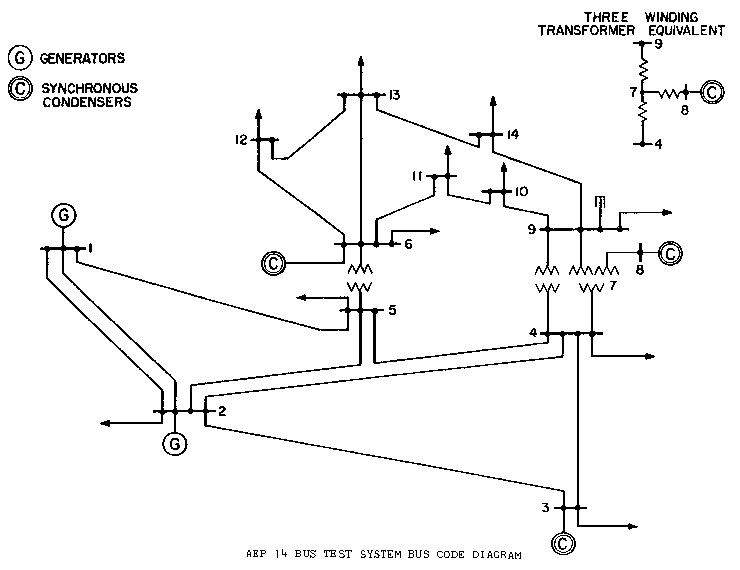
\includegraphics[width=10cm]{figuras/14bus.jpg} 
\label{FigRede14barras}
\end{figure}

\subsection{Solução por software}
É possivel notar que com tolerância = $0.000001pu$, a rede convergiu para solução em 4 iterações, em $0.39s$
\begin{minted}[mathescape, style = autumn,
    frame = single, fontsize=\footnotesize]{matlab}
> Relatório final
  Convergiu em 4 iterações
> Estado da rede
Barra Tipo       Mag   Fase         P       Q       Qsh
  1    3    1.0000  -0.00    4.9041 -0.5519    0.0000 
  2    2    1.0000 -12.32   -0.2170  1.5340    0.0000 
  3    2    1.0000 -24.46   -0.9420  0.7185    0.0000 
  4    0    0.9301 -23.23   -0.4780  0.0390    0.0000 
  5    0    0.9300 -20.79   -0.0760 -0.0160    0.0000 
  6    2    1.0000 -41.97   -0.1120  0.9492    0.0000 
  7    0    0.9434 -34.85   -0.0000  0.0000    0.0000 
  8    2    1.0000 -34.85    0.0000  0.3212    0.0000 
  9    0    0.9304 -40.93   -0.2950 -0.1660    0.1645 
 10    0    0.9014 -46.00   -0.9000 -0.0580    0.0000 
 11    0    0.9289 -46.05   -0.3500 -0.0180    0.0000 
 12    0    0.9206 -47.88   -0.6100 -0.0160    0.0000 
 13    0    0.9593 -44.41   -0.1350 -0.0580    0.0000 
 14    0    0.9225 -43.72   -0.1490 -0.0500    0.0000 

> Fluxos de potência
 De Para       Pkm     Qkm       Pmk     Qmk     Ploss   Qloss
  1    5    1.5319  0.1897   -1.4026  0.2981    0.1293  0.4878
  1    2    3.3722 -0.7416   -3.1419  1.3920    0.2303  0.6503
  2    5    0.8477  0.1660   -0.8049 -0.0675    0.0428  0.0985
  2    4    1.0464  0.1297   -0.9816  0.0355    0.0649  0.1652
  2    3    1.0307 -0.1537   -0.9800  0.3236    0.0507  0.1700
  3    4    0.0380  0.3949   -0.0274 -0.3680    0.0105  0.0269
  4    5   -0.7876  0.2713    0.7983 -0.2375    0.0107  0.0338
  4    7    0.8454  0.0269   -0.8454  0.1460    0.0000  0.1729
  4    9    0.4732  0.0733   -0.4732  0.0741    0.0000  0.1474
  5    6    1.3333 -0.0091   -1.3333  0.5271    0.0000  0.5180
  6   12    0.4295  0.1233   -0.4049 -0.0722    0.0245  0.0511
  6   13    0.3778  0.1271   -0.3673 -0.1064    0.0105  0.0207
  6   11    0.4139  0.1717   -0.3949 -0.1317    0.0191  0.0399
  7    9    0.8454  0.1570   -0.8454 -0.0656    0.0000  0.0914
  7    8    0.0000 -0.3030    0.0000  0.3212    0.0000  0.0182
  9   10    0.8854  0.0242   -0.8566  0.0524    0.0288  0.0766
  9   14    0.1382 -0.0342   -0.1352  0.0406    0.0030  0.0063
 10   11   -0.0434 -0.1104    0.0449  0.1137    0.0014  0.0033
 12   13   -0.2051  0.0562    0.2168 -0.0456    0.0118  0.0107
 13   14    0.0155  0.0940   -0.0138 -0.0906    0.0017  0.0034
> Tempo computacional =  0.3942 segundos.
\end{minted}




\chapter{C\'odigo comentado}
\label{SectionCodigo}

Os códigos fonte desse trabalho bem como histórico de modificação, podem ser encontrados no endereço: \textit{\href{https://github.com/phneves/ElectricPowerSystemsAnalysisTools}{https://github.com/phneves/ElectricPowerSystemsAnalysisTools}}.
\section{Entradas e configurações}
Iniciamos com limpeza das variáveis no \textit{workspace} e da tela. Também há configurações do script.
\begin{minted}[mathescape, style = autumn,
    frame = single, fontsize=\footnotesize]{matlab}
clear all;
clc;
tol = 0.00001; 
% Arquivo de dados da rede
%P2GTD
RedePequena
graf = 'nao'; % Mostrar graficos ao final do cálculo
itmax = 20;% Número máximo de iterações permitido
% Tensões mínima e máxima permitidas
vmin = 0.0;
vmax = 2.0;
% Considerar cargas dependentes da tensão?
% 'nao'->modelo de pot cte. 'sim'->ModeloCarga deve ser especificado
cargasV = 'nao';
graus_to_rad = pi/180;% Conversão graus <-> radianos
rad_to_graus = 180/pi;
Debug = true; %pneves: Enable debug prints.
\end{minted}
%%%%%%%%%%%%%%%%%%%%%%%%%%%%%%%%%%%%%%%%%%%%%%%%%%%%%%
Carrega-se então, os valores da rede nas variáveis apropriadas. Vetores receberão dados das barras.
\begin{minted}[mathescape, style = autumn,
    frame = single, fontsize=\footnotesize]{matlab}
%Número - Tipo - V - Ângulo - Pg - Qg - Pc - Qc - bshk
for k = 1:nb            %pneves: extracting bar values into arrays
    numext(k)   = barras(k,1);                  
    tipo(k)     = barras(k,2);                  
    v(k)        = barras(k,3);                  
    ang(k)      = barras(k,4) * graus_to_rad;   
    pg(k)       = barras(k,5)/baseMVA; %pneves: PU 
    qg(k)       = barras(k,6)/baseMVA;
    pc(k)       = barras(k,7)/baseMVA;
    qc(k)       = barras(k,8)/baseMVA;
    bshk(k)     = barras(k,9)/baseMVA;
        pnom(k)     = pg(k) - pc(k); %pneves: P liquido
        qnom(k)     = qg(k) - qc(k); %pneves: Q liquido
    numint(barras(k,1)) = k;
end
\end{minted}
%%%%%%%%%%%%%%%%%%%%%%%
Vetores receberão dados dos ramos.
%FALAR COMO É CALCULADO OS MISMATCHES
\begin{minted}[mathescape, style = autumn,
    frame = single, fontsize=\footnotesize]{matlab}
for l = 1:nr                %	Carregamento dos vetores de ramo
	de(l)   = ramos(l,1);
	para(l) = ramos(l,2);
	r(l)    = ramos(l,3);
	x(l)    = ramos(l,4);
	bshl(l) = ramos(l,5)/2.; %shunt aqui é dividido por 2
	tap(l)  = ramos(l,6);
	fi(l)   = 0; %- ramos(l,7) * graus_to_rad;
end
fprintf('\n> Modelo de carga: potência constante (default).\n')
\end{minted}
%%%%%%%%%%%%%%%%%%%%%%%%%%%%%%%%%%%%%%%%%%%%%%%%
Neste ponto do código, será criada a matriz de admitância. A regra de formação dessa matriz está descrita em \ref{AdmitanciaElementosForaDiagonal} e \ref{AdmitanciaElementosDiagonal}. 
\begin{minted}[mathescape, style = autumn,
    frame = single, fontsize=\footnotesize]{matlab}
%pneves: Matriz Y dimensionada para NBxNB
Y = zeros(nb,nb);
for k = 1:nb
    Y(k,k) = i*bshk(k); %pneves: Cada Y(k,k) recebe 0+i*shunt
end
\end{minted}
%%%%%%%%%%%%%%%%%%%%%%%%%%%%%%%%%%%%%%%%%%%%%%
Preenchimento da matriz admitância.
\begin{minted}[mathescape, style = autumn,
    frame = single, fontsize=\footnotesize]{matlab}
for l = 1:nr %pneves: As formulas de formação da matriz
    k = de(l)%estão no Tópico Matriz de Admitância  
    m = para(l)
    y(l) = 1/(r(l) + i*x(l))
    akk(l) = 1/(tap(l)*tap(l))
    amm(l) = 1.0
    akm(l) = 1/tap(l)
    Y(k,k) = Y(k,k) + akk(l)*y(l) + i*bshl(l)
    Y(m,m) = Y(m,m) + amm(l)*y(l) + i*bshl(l)
    Y(k,m) = Y(k,m) - akm(l)*y(l)
    Y(m,k) = Y(m,k) - akm(l)*y(l)
end
G = real(Y); %pneves: matriz de condutância 
B = imag(Y); %pneves: matriz de susceptância
if (Debug == true) %pneves: Debug
    fprintf('DEBUG> Y, G and B complete\n');
    Y
    G
    B
end
\end{minted}
Aqui será definido o estado inicial da rede, com $V = 1$ PU para barras $PQ$, com $\theta = 0$ para barras $PQ$ e $PV$. O chamado \textit{Flat guess}.
\begin{minted}[mathescape, style = autumn,
    frame = single, fontsize=\footnotesize]{matlab}
for k = 1:nb
    if tipo(k) ~= 3
        ang(k) = 0.0;
        if tipo(k) < 2
            v(k)= 1.0;
        end
    end
end
\end{minted}

\section{Subsistema 1 - Iterativo}
Calcula-se as Potências nodais.\\
$pcalc(k)$ e $qcalc(k)$ são calculados para cada barra. Eles serão usados nos calculos de $H_{kk}$, $N_{kk}$, $M_{kk}$ e $L_{kk}$, submatrizes da matriz Jacobiana \ref{Jacobiana}.\\
\begin{minted}[mathescape, style = autumn,
frame = single, fontsize=\footnotesize]{matlab}
iter = 0;       %	Inicializar contador de iterações
maxDP = 10^5;   %	Inicializar maiores mismatches
maxDQ = 10^5;   
while abs(maxDP) > tol | abs(maxDQ) > tol %	Processo iterativo 
    %Cálculo das potências nodais
    for k = 1:nb
        pcalc(k) =  G(k,k)*v(k)*v(k);
        qcalc(k) = -B(k,k)*v(k)*v(k);
    end
    for l = 1:nr
        k = de(l);
        m = para(l);
        ab = ang(k) - ang(m) + fi(l);
        gkm = akm(l)*real(y(l));
        bkm = akm(l)*imag(y(l));
        pcalc(k) = pcalc(k) + v(k)*v(m)*(-gkm*cos(ab)-bkm*sin(ab));
        pcalc(m) = pcalc(m) + v(k)*v(m)*(-gkm*cos(ab)+bkm*sin(ab));
        qcalc(k) = qcalc(k) + v(k)*v(m)*(-gkm*sin(ab)+bkm*cos(ab));
        qcalc(m) = qcalc(m) - v(k)*v(m)*(-gkm*sin(ab)-bkm*cos(ab));
    end
\end{minted}
%%%%%%%%%%%%%%%%%%%%%%%
%FALAR DE ONDE VEM OS PCALC, QCALC. QUAL EQUAÇÃO AQUI ELES SE RELACIONAM
%FALAR COMO É CALCULADO OS MISMATCHES
As equações de $pcalc(k)$ (bloco de código acima) são termos somatórios descritas nas equações \ref{H_resolvido}, \ref{N_resolvido}, \ref{M_resolvido} e \ref{L_resolvido}.\\
No bloco de código abaixo, tem-se o cáculo dos \textit{mismatches} de potência (P e Q).
\begin{equation}
\left\{    \begin{array}{lll}
                DP(k)=pesp(k)-pcalc(k)\\
                DQ(k)=qesp(k)-qcalc(k)
            \end{array}\right.
    \label{DePcalc}
\end{equation}
As equações descritas em \ref{DePcalc} são as diferenças entre as potências esperadas e as calculadas, respectivamente para P e Q.\\
Esses valores serão os novos $\Delta P$ e $\Delta Q$, como descrito na equação \ref{delta_x_nu}.\\
No bloco subsequente, a variável de controle do número de iteração é incrementada. Neste algorítmo, $\nu$ está descrito como \textit{iter}.\\
O vetor $DS$ é montado. 
%\newpage
\begin{minted}[mathescape, style = autumn,
    frame = single, fontsize=\footnotesize]{matlab}
    %Cálculo dos mismatches de potência
    DP = zeros(nb,1);
    DQ = zeros(nb,1);
    maxDP = 0;
    maxDQ = 0;
    busDP = 0;
    busDQ = 0;
    for k = 1:nb
        pesp(k) = pnom(k);
        qesp(k) = qnom(k);
        if tipo(k) ~= 3
            DP(k) = pesp(k) - pcalc(k);
            if abs(DP(k)) > abs(maxDP)
                maxDP = DP(k);
                busDP = numext(k);
            end
        end
        if tipo(k) <= 1
            DQ(k) = qesp(k) - qcalc(k);
            if abs(DQ(k)) > abs(maxDQ)
                maxDQ = DQ(k);
                busDQ = numext(k);
            end
        end
    end
\end{minted}
%%%%%%%%%%%%%%%%%%%%%%%%%%%%%%%%%%%%%%%%%%%%%%%%%%%%
\begin{minted}[mathescape, style = autumn,
    frame = single, fontsize=\footnotesize]{matlab}
    iteracao(iter+1) = iter;
    mismP(iter+1) = abs(maxDP);
    mismQ(iter+1) = abs(maxDQ);

    DS = [ DP ; DQ ];

    fprintf('\n> Iteração - %d\n',iter)
    fprintf('* Máximo mismatch P = %06.4f (barra %04d)\n',maxDP,busDP)
    fprintf('* Máximo mismatch Q = %06.4f (barra %04d)\n',maxDQ,busDQ)
\end{minted}
Caso o \textit{mismatch} seja maior que a tolerância, a matriz Jacobiana será montada e o estado será atualizado.
\begin{minted}[mathescape, style = autumn,
    frame = single, fontsize=\footnotesize]{matlab}
    if abs(maxDP) > tol | abs(maxDQ) > tol
        %	Montar e inverter a matriz Jacobiana
        H = zeros(nb,nb); M=H; N=H; L=H;
        for k = 1:nb
            H(k,k) = -qcalc(k) - v(k)*v(k)*B(k,k);
            if tipo(k) == 3
                H(k,k) = 10^10;
            end
            N(k,k) = ( pcalc(k) + v(k)*v(k)*G(k,k) )/v(k) ;
            M(k,k) = pcalc(k) - v(k)*v(k)*G(k,k);
            L(k,k) = ( qcalc(k) - v(k)*v(k)*B(k,k) )/v(k) ;
            if tipo(k) >= 2
                L(k,k) = 10^10;
            end
        end
        for l = 1 : nr,
              k = de(l) ;
              m = para(l) ;
              ab = ang(k) - ang(m) + fi(l) ;
                
              H(k,m) =   v(k)*v(m)*( G(k,m)*sin(ab)-B(k,m)*cos(ab)) ;
              H(m,k) =   v(k)*v(m)*(-G(k,m)*sin(ab)-B(k,m)*cos(ab)) ;
              N(k,m) =   v(k)*(G(k,m)*cos(ab)+B(k,m)*sin(ab)) ;
              N(m,k) =   v(m)*(G(k,m)*cos(ab)-B(k,m)*sin(ab)) ;
              M(k,m) = - v(k)*v(m)*(G(k,m)*cos(ab)+B(k,m)*sin(ab)) ;
              M(m,k) = - v(k)*v(m)*(G(k,m)*cos(ab)-B(k,m)*sin(ab)) ;
              L(k,m) =   v(k)*(G(k,m)*sin(ab)-B(k,m)*cos(ab)) ;
              L(m,k) = - v(m)*(G(k,m)*sin(ab)+B(k,m)*cos(ab)) ;
        end
        J = [ H N ; M L ];
        %	Calcular o vetor de correção de estado
        DV = inv(J)*DS;
        %	Atualizar estado
        v = v + DV(nb+1:2*nb)';
        ang = ang + DV(1:nb)';
        
\end{minted}
%%%%%%%%%%%%%%%%%%%%%%%
Verifica-se se há divergência, ou seja, se o método está caminhando para uma resposta. 
\begin{minted}[mathescape, style = autumn,
    frame = single, fontsize=\footnotesize]{matlab}
        %	Verificar se houve divergência
        for k = 1:nb
            if v(k) < vmin | v(k) > vmax
                fprintf('\n> Tensões fora dos limites ->
                divergência.\n')
                fprintf('> Execução interrompida.\n\n')
                if graf == 'sim'
                            graficos
                end
                msgbox('Tensões fora dos limites -> divergência.
                Execução interrompida.','Aviso','warn');
                return
            end
        end
\end{minted}
%%%%%%%%%%%%%%%%%%%%%%%
Verifica-se se o método excedeu o número de iterações máximas.
\begin{minted}[mathescape, style = autumn,
    frame = single, fontsize=\footnotesize]{matlab}
    %	Incrementar contador de iterações

    iter = iter + 1;

        if iter > itmax
            fprintf('\n> Número máximo de iterações permitido foi
            excedido.\n')
            fprintf('> Execução interrompida.\n\n')
            if graf == 'sim'
                graficos
            end
            msgbox('Número máximo de iterações permitido foi
            excedido. Execução interrompida.','Aviso','warn');
            return
        end
    end
end	% final do while
\end{minted}
\section{Subsistema 2 - Cálculo de $P_k$ e $Q_k$}
Neste ponto, o software já fez todos os calculos e se saiu do laço de repetição \textit{while}, então ele convergiu para resposta.\\
As potências serão recalculadas com os valores finais para gerar o relatório.
\begin{minted}[mathescape, style = autumn,
    frame = single, fontsize=\footnotesize]{matlab}
%%
%'Fim do cálculo de fluxo de carga. Preparando relatório de saída');
fprintf('\n> Fim do cálculo de fluxo de carga. 
Preparando relatório de saída ...\n')
\end{minted}
Será calculada as potências nodais.
\begin{minted}[mathescape, style = autumn,
    frame = single, fontsize=\footnotesize]{matlab}
%	Cálculo das potências nodais
for k = 1:nb
	pcalc(k) = G(k,k)*v(k)*v(k);
    qcalc(k) = -B(k,k)*v(k)*v(k);
end
for l = 1:nr
	k = de(l);
    m = para(l);
    ab = ang(k) - ang(m) + fi(l);
    gkm = akm(l)*real(y(l));
    bkm = akm(l)*imag(y(l));
    pcalc(k) = pcalc(k) + v(k)*v(m)*(-gkm*cos(ab)-bkm*sin(ab));
    pcalc(m) = pcalc(m) + v(k)*v(m)*(-gkm*cos(ab)+bkm*sin(ab));
    qcalc(k) = qcalc(k) + v(k)*v(m)*(-gkm*sin(ab)+bkm*cos(ab));
    qcalc(m) = qcalc(m) - v(k)*v(m)*(-gkm*sin(ab)-bkm*cos(ab));
end
\end{minted}
Será calculado o fluxo de potência nos ramos
\begin{minted}[mathescape, style = autumn,
    frame = single, fontsize=\footnotesize]{matlab}
%	Cálculo dos fluxos de potência nos ramos
for l = 1:nr
    k = de(l);
    m = para(l);
    gkm = real(y(l));
    bkm = imag(y(l));
    ab = ang(k) - ang(m) + fi(l);
    vkm = v(k)*v(m);
    pkm(l) = akk(l)*v(k)*v(k)*gkm -
        akm(l)*vkm*(gkm*cos(ab)+bkm*sin(ab));
    pmk(l) = amm(l)*v(m)*v(m)*gkm -
        akm(l)*vkm*(gkm*cos(ab)-bkm*sin(ab));
    qkm(l) = -akk(l)*v(k)*v(k)*(bkm+bshl(l)) +
        akm(l)*vkm*(bkm*cos(ab)-gkm*sin(ab));
    qmk(l) = -amm(l)*v(m)*v(m)*(bkm+bshl(l)) +
        akm(l)*vkm*(bkm*cos(ab)+gkm*sin(ab));
    pperdas(l) = pkm(l) + pmk(l);
    qperdas(l) = qkm(l) + qmk(l);
end
\end{minted}
Apresentação do relatório final. 
\begin{minted}[mathescape, style = autumn,
    frame = single, fontsize=\footnotesize]{matlab}
fprintf('\n\n> Relatório final\n\n') %	Relatório final
fprintf('  Convergiu em %d iterações\n\n',iter)
fprintf('> Estado da rede\n\n')
fprintf('   Barra Tipo   Mag Fase    P   Q   Qsh\n')
for k = 1:nb
    fprintf('%7d %4d %9.4f %6.2f %9.4f %7.4f %9.4f \n',
    numext(k),tipo(k),v(k),(ang(k)*rad_to_graus),pcalc(k),
    qcalc(k), bshk(k)*v(k)^2)
end
fprintf('\n> Fluxos de potência\n\n')
fprintf('   De  Para    Pkm   Qkm   Pmk   Qmk Ploss   Qloss\n')
for l = 1:nr
    fprintf('%7d %4d %9.4f %7.4f %9.4f %7.4f %9.4f %7.4f\n',
    de(l),para(l),pkm(l),qkm(l),pmk(l),qmk(l),pperdas(l),qperdas(l))
end
if graf == 'sim'
    graficos
end
tempo = toc; % terminando contagem de tempo computacional
fprintf('\n\n> Tempo computacional = %7.4f segundos.',tempo)
fprintf('\n\n> Fim da simulação.\n\n')
\end{minted}

\section{Método de Newton Desacoplado}
Para os métodos desacoplados, haverá modificações na matriz Jacobiana. Portanto todo o código será o mesmo, com excessão das partes que montam essa matriz, que é baseada em \ref{HNML_eq_rapido}.\\ 
Nesse trecho de código, as matrizes $M$ e $N$ são zeradas, para demonstrar que não serão utilizadas, mas para ganho de performance, essas matrizes não são calculadas nos Métodos desacoplados.
\begin{minted}[mathescape, style = autumn,
    frame = single, fontsize=\footnotesize]{matlab}
    N = zeros(nb,nb);
    M = zeros(nb,nb);
    J = [ H N ; M L ]
\end{minted}

\section{Método de Newton desacoplado rápido} 
Para o método desacoplado rápido, a formação da matriz Jacobiana seguirá como descrito em \ref{Blinha} e \ref{Bduaslinhas}. Note que é bem mais simples de calcular, após todas as simplificações.
\begin{minted}[mathescape, style = autumn,
    frame = single, fontsize=\footnotesize]{matlab}
for l = 1 : nr,
      k = de(l) ;
      m = para(l) ;

      ab = ang(k) - ang(m) + fi(l) ;
      
      %pneves:fast version. Slide Pag38
      H(k,m) =   -B(k,m);
      H(m,k) =    B(k,m);
      %N(k,m) =   v(k)*(G(k,m)*cos(ab)+B(k,m)*sin(ab)) ;
      %N(m,k) =   v(m)*(G(k,m)*cos(ab)-B(k,m)*sin(ab)) ;
      %M(k,m) = - v(k)*v(m)*(G(k,m)*cos(ab)+B(k,m)*sin(ab)) ;
      %M(m,k) = - v(k)*v(m)*(G(k,m)*cos(ab)-B(k,m)*sin(ab)) ;
      L(k,m) =   -B(k,m);
      L(m,k) =   -B(k,m);
end
\end{minted}

\chapter{Discussões e an\'alise de resultados}


%\include{ex5}

%\include{ex6}

% Os comandos para incluir as referências bibliográficas
\begin{singlespacing}
\setlength\bibitemsep{10pt}   % Adiciona uma linha em branco entre duas referências
\printbibliography[heading=bibintoc, % Adiciona no sumário
                   title={Referências bibliográficas} % Nome do Capítulo
                  ]
\end{singlespacing}

% Os anexos, se houver, vêm depois das referências:
%\appendix

% O comando a seguir inclui o arquivo apendices.tex
% que contém os apêndices. Observe o comando \appendix
% na linha anterior
% Detalhe: não precisa incluir a extensão .tex
%\include{apendices}

\end{document}